The algorithm is relatively simple for this proof of concept. There are two main steps of the algorithm: the pre-processing of the input image, and the matching of two images.

\subsection{Pre-processing}

The image that was uploaded to the system is considered the raw image. There are limitations about the original image, including

\begin{itemize}
	\item the lighting situation might change throughout the day;
	\item the position of the camera might vary;
	\item the muzzle lines are hard to detect as they tend to be of darker colour...
\end{itemize}

To tackle those problems the image needs to undergo a pre-processing step that will filter out the parts that are not related to muzzle lines and will potentially tamper our recognition process.

The first step is to read the image into the system. Instead of using the RGB colourspace we decided to use HSV instead, and one of the reasons of doing so is that so it would be easier to ignore the "lightness" factor from the image\footnote{Because then we would be able to normalise the image on V - Value, which is also called lightness of an image.} by normalising on the lightness (See fig~\ref{fig:original}).

We then need to convert the image to grayscale to speed up the future process (as we essentially just trimmed the size of the matrix representing the muzzle image to a third of it originally) and then apply the Sobel operator (to find the edges of the image; see fig~\ref{fig:grayscale}).

The next step is to apply a (dynamic) threshold to make the image into binary (see fig~\ref{fig:binary}).

Then to remove the circles surrounded by lines we need to dilate and erode the image. The reason of doing so is that based on our discovery it is very rare for the muzzle to have (small) closed circles on it (see fig~\ref{fig:dilate_and_erode}).

\subsection{Matching}

The matching process includes two steps: to find a way to describe the important bits for matching mathematically of an image and to actually match two of them.

For this exercise we have decided to use the Harris Corner Detector for detecting features, ORB descriptor \cite{orb} for describing the features mathematically. For detecting the similarity of two images, we have decided to use a brute-force hamming distance matcher \cite{feature_matching} for calculating the distance between two muzzles - the greater the distance is, the less similar the two images are.

\begin{figure}[H]
  	\centering
    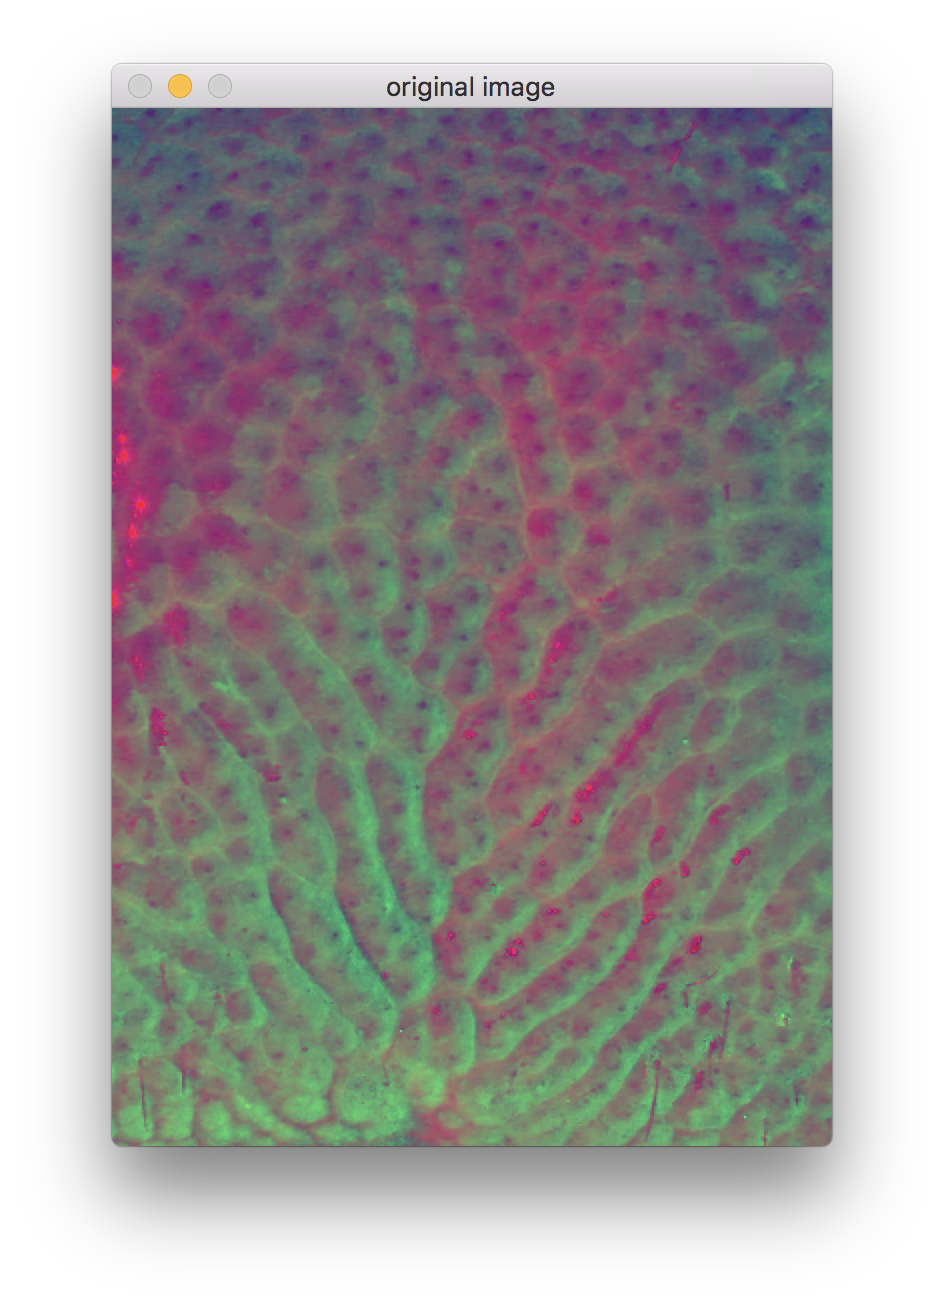
\includegraphics[width=0.4\textwidth]{images/algorithm/original.png}
    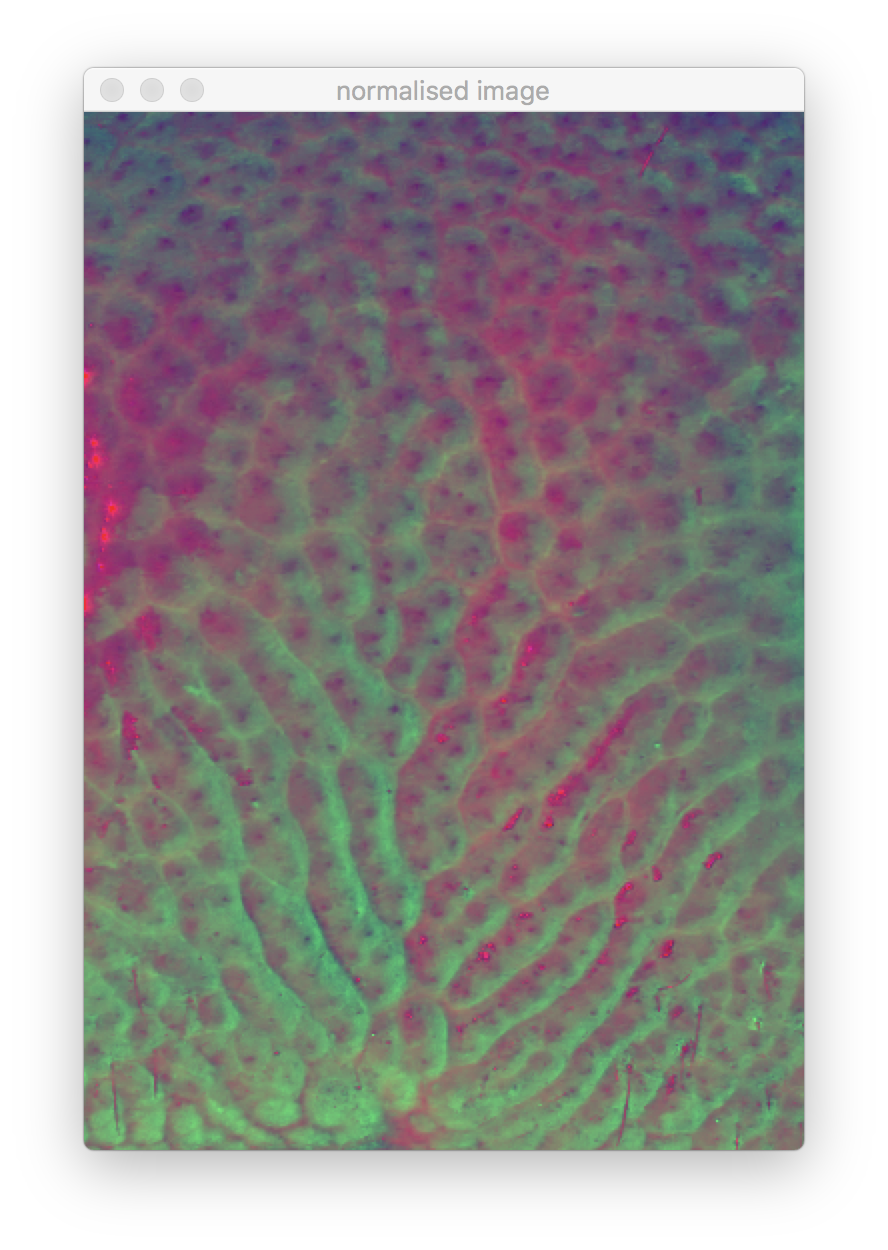
\includegraphics[width=0.4\textwidth]{images/algorithm/normalised.png}

  	\caption[Original and Normalised Image]{Original and Normalised Image}
  	\label{fig:original}
\end{figure}

\begin{figure}[H]
  	\centering
    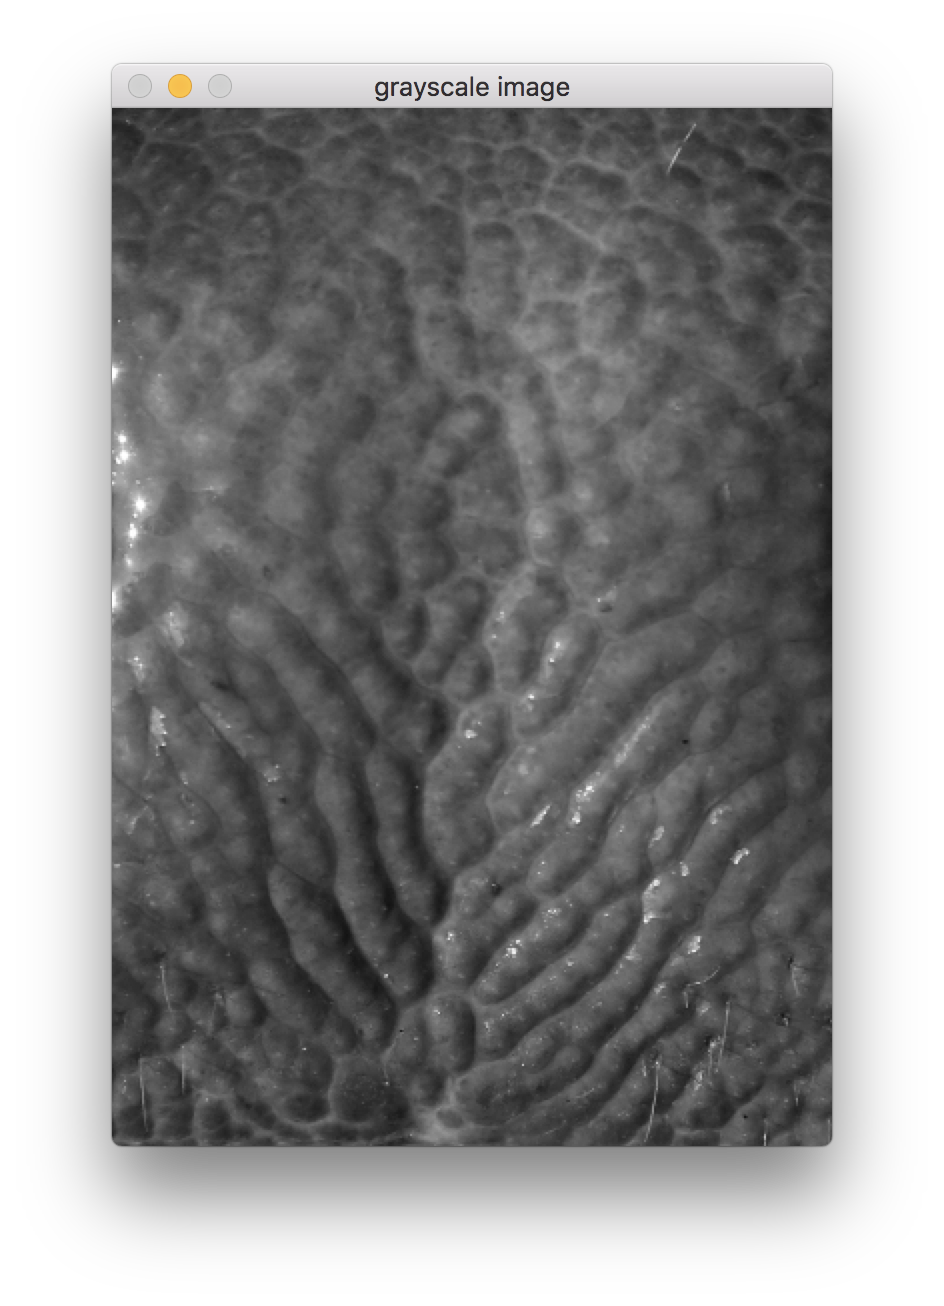
\includegraphics[width=0.4\textwidth]{images/algorithm/grayscale.png}
    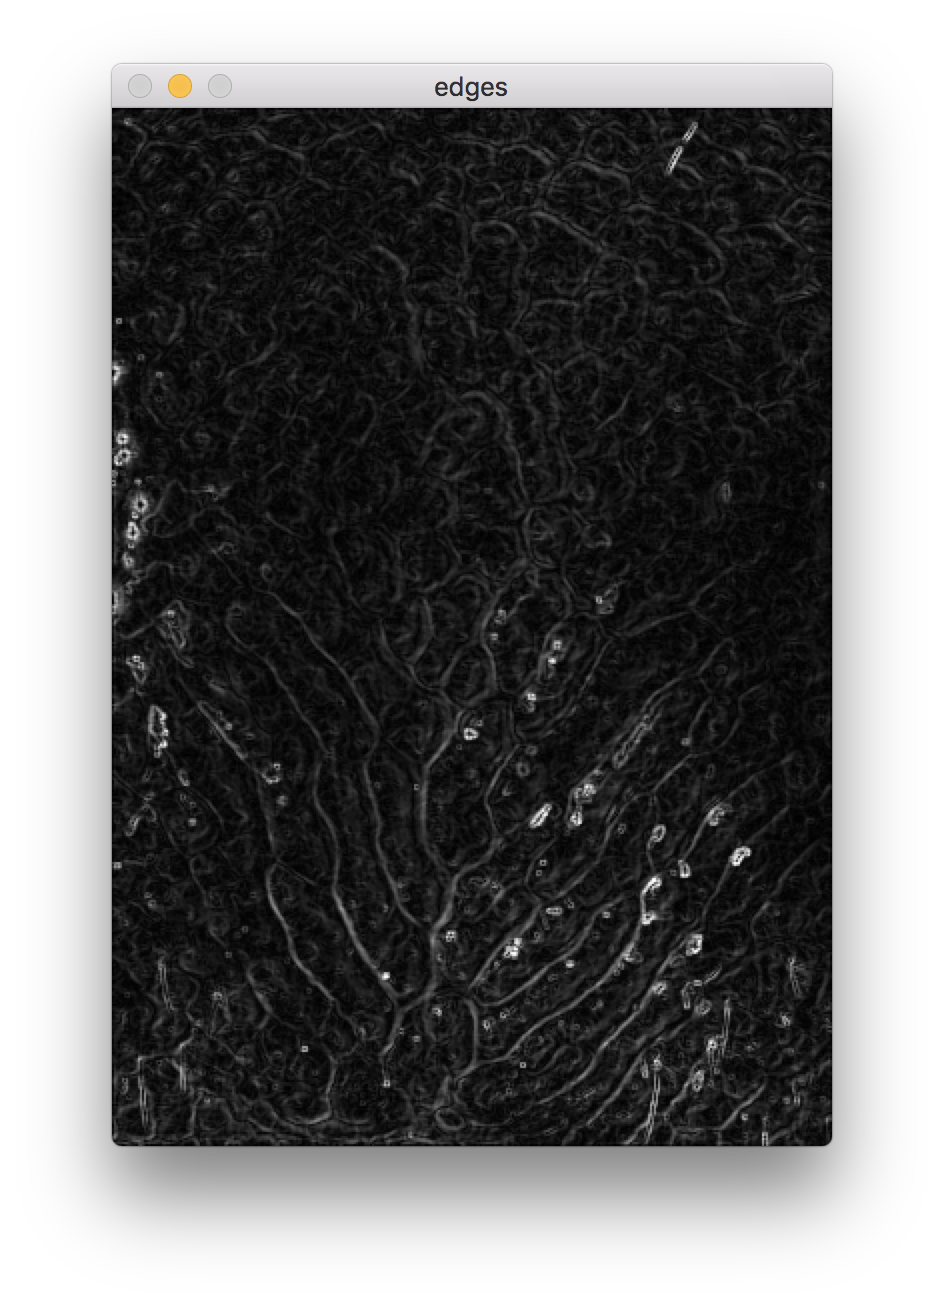
\includegraphics[width=0.4\textwidth]{images/algorithm/edges.png}

  	\caption[Grayscale Image and Its Edges]{Grayscale Image and Its Edges}
  	\label{fig:grayscale}
\end{figure}


\begin{figure}[H]
  	\centering
    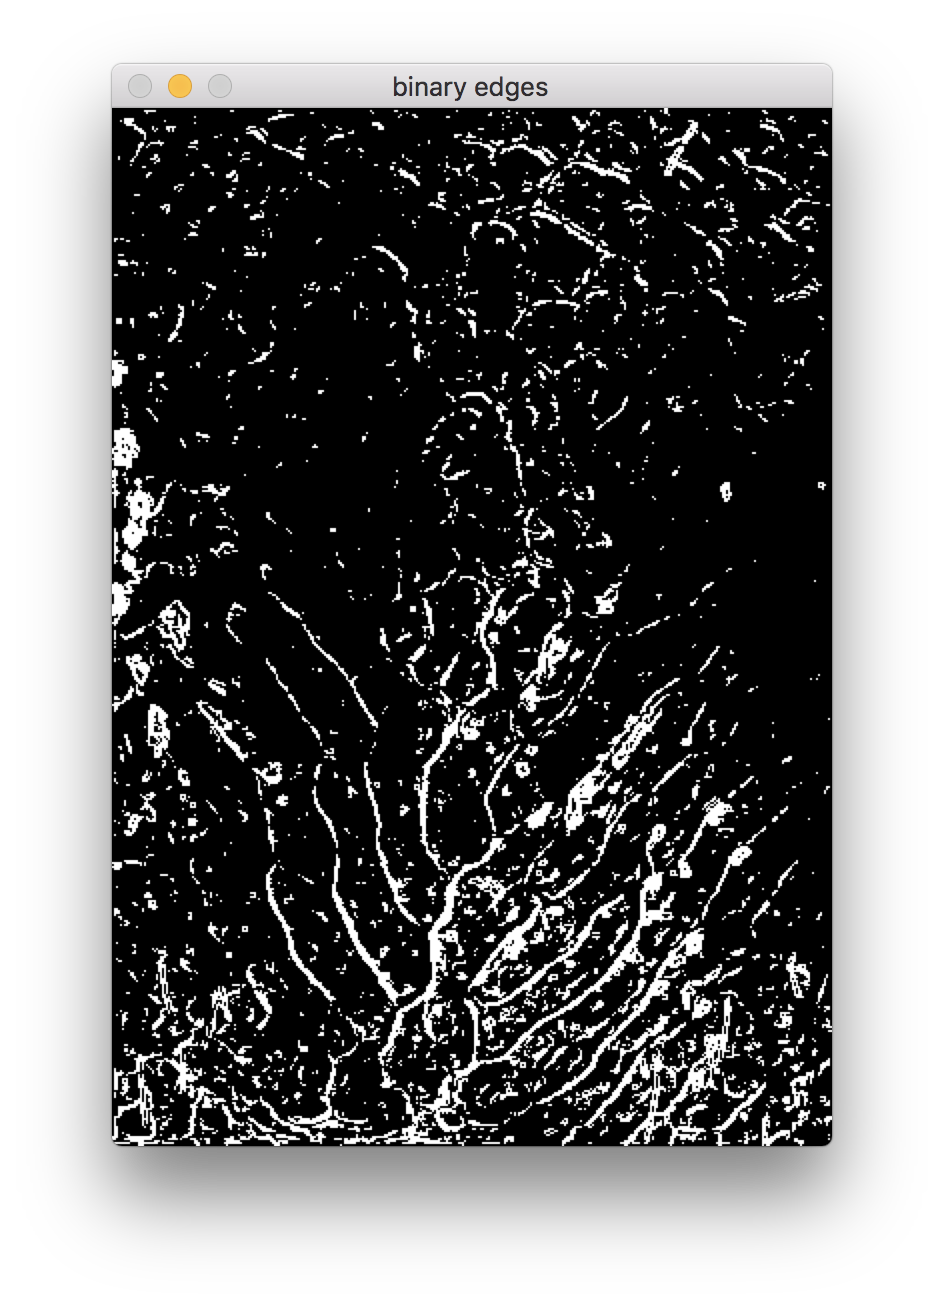
\includegraphics[width=0.4\textwidth]{images/algorithm/binary.png}

  	\caption[Binary Image]{Binary Image}
  	\label{fig:binary}
\end{figure}


\begin{figure}[H]
  	\centering
    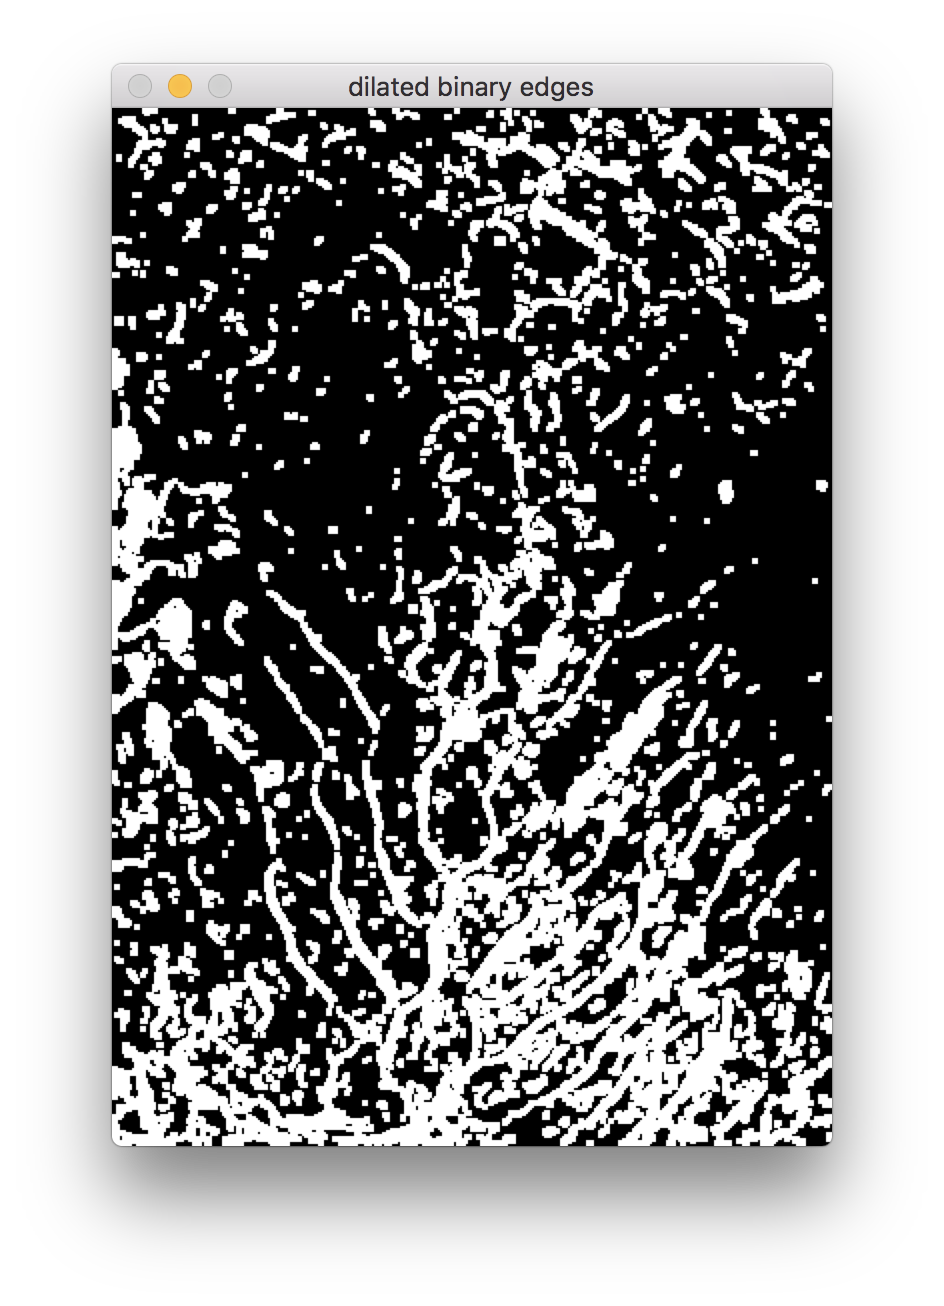
\includegraphics[width=0.4\textwidth]{images/algorithm/dilated.png}
    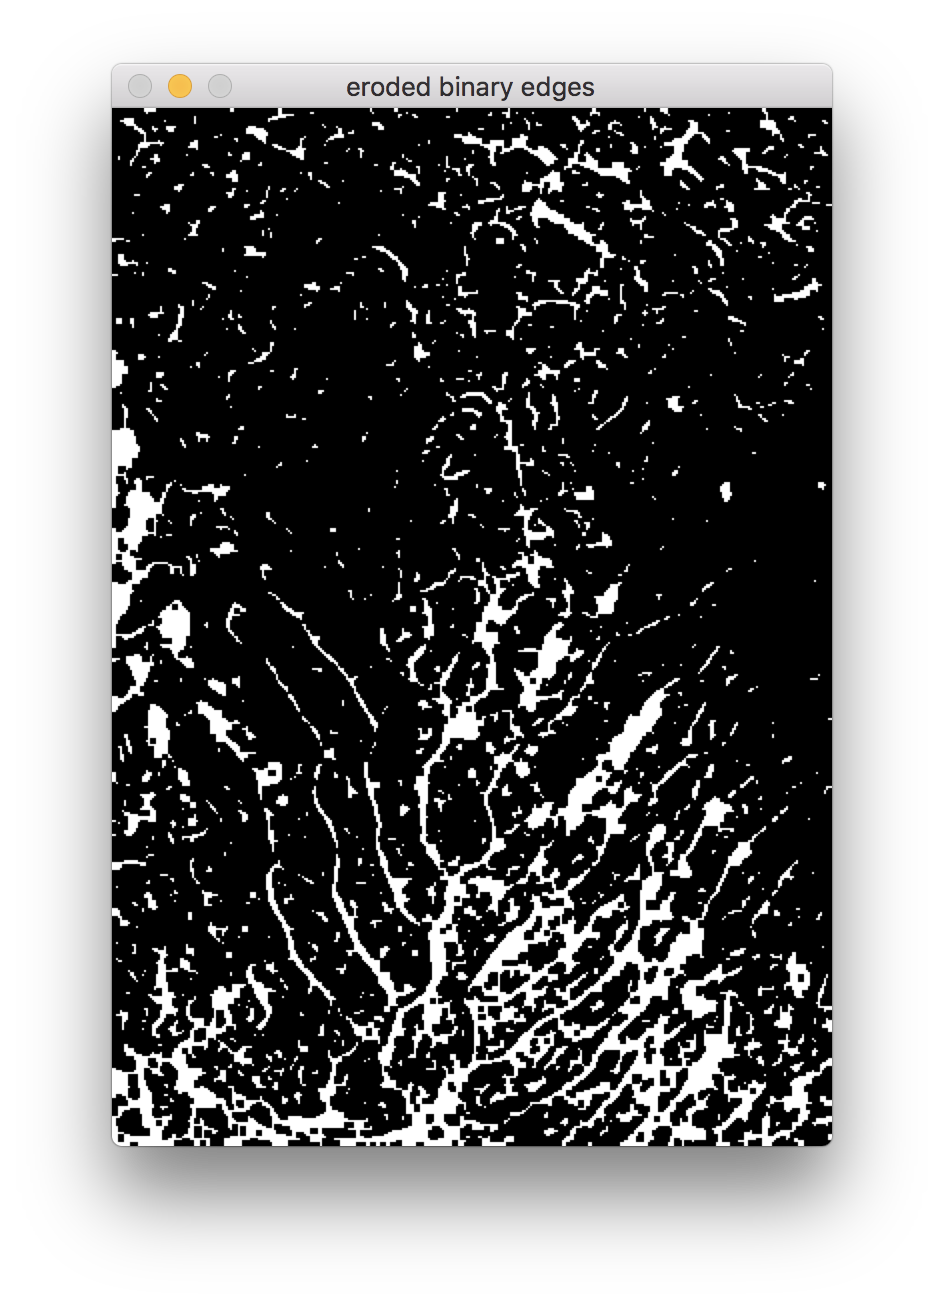
\includegraphics[width=0.4\textwidth]{images/algorithm/eroded.png}

  	\caption[Dilated and Eroded Image]{Dilated and Eroded Image}
  	\label{fig:dilate_and_erode}
\end{figure}
